\chapter*{TrackNTrace}
TrackNTrace is a fast, easy-to-use Matlab program created for locating bright, Gaussian-shaped spots in a 2D fluorescence microscopy image or movie and track such emitters over time. It can be used in localization microscopy (PALM, STORM, ...), Single-molecule Particle Tracking (SPT), for drift correction and similar applications and comes with a convenient interface for configuration. Locating and tracking fluorescent emitters is done in two separate steps and it is comparatively easy for anyone with basic Matlab knowledge to alter the respective scripts, e.g. to include additional tracking algorithms. TrackNTrace should be useful to anyone who seeks to combine the speed of established software packages like RapidSTORM or quickPALM with the simplicity and direct modifiablity of Matlab, especially when further post-processing is also done in Matlab.\\
In general, TrackNTrace reads a movie file, corrects for camera artifacts if applicable and obtains a rough guess of all possible positions of bright spots in every image. These position candidates then serve as the basis for a fitting routine which fits a 2D Gaussian bell curve to the pixel intensity values around each candidate as an approximation of the microscope Point Spread Function (PSF), obtaining position, amplitude and local background. Finally, these fit results are then returned to a particle tracking algorithm which tries to link particles close in time and space to get their trajectories.\\[10pt]
This manual will first provide all necessary steps for installation (section~\ref{sec:install}) and explain the configuration utility (section~\ref{sec:config}). Some in-depth information about the operation of TrackNTrace is provided in section~\ref{sec:indepth}.

\begin{table}
\centering
\caption*{\textbf{Requirements}}
\label{tab:requirements}
\begin{tabular}{p[.15\textwidth] p[.45\textwidth]}
\toprule
OS & Windows 7x64 or higher\footnote{Necessary libraries can also be compiled for Linux and Mac.} \\
Matlab version & 2009a or higher\\
Toolbox & Image Processing, Statistics
\bottomrule
\end{tabular}
\end{table}
Please also note: TrackNTrace currently can only handle single-channel, 2D+t Tif image stacks. Convert your experimental data accordingly.

\section{Installation}\label{sec:install}
Installation procedure for Windows 7:
\begin{enumerate}
\item Extract TrackNTrace.zip to your Matlab root path directory (e.g. \url{C:\\Users\\\%USERNAME\%\\Documents\\MATLAB}).
\item Open the TrackNTrace folder and run \texttt{vcredist_x64.exe}.
\item Open Matlab and add the TrackNTrace folder to your Matlab path.
\item Run \texttt{RunTrackNTrace.m}.
\end{enumerate}

\section{Configuration}\label{sec:config}
When you first run \texttt{RunTrackNTrace.m}, the GUI as seen in figure~\ref{fig:settings_gui} pops up. Here, you can select the relevant movie files to process, set options to find spots and fit a PSF model to them, and handle the particle tracking algorithms. All relevant file names, options, particle locations, and trajectories are stored in a time-stamped \texttt{mat}-file whenever they become available which makes it very easy to repeat and compare different experiments and very hard to lose any progress. Before processing begins, users can enable a preview mode to try and optimize different settings, either individually for all selected movies or globally. Finally, finished movies can be inspected in Matlab with trajectories overlaid.

\begin{figure}[!h]
\centering
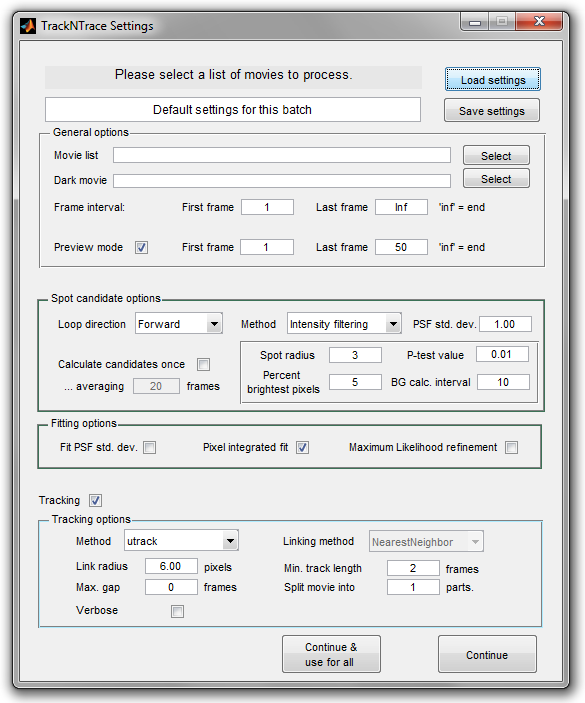
\includegraphics[width=5cm]{./settings_gui_first.png}
\caption{GUI for TrackNTrace settings.}
\label{fig:settings_gui}
\end{figure}

You can always save the current settings in a different \texttt{mat}-file and load them at the start by clicking on \textit{Save Settings} and \textit{Load settings}, respectively. In such a case, one only needs to select the movies to process and can skip anything else. Clicking on \textit{Continue \& use for all} will use the same settings for all selected movies while clicking \textit{Continue} allows to change settings for each individual movie.

\subsection*{General options}
\begin{itemize}
\item[Movie list] Click on \textit{Select} to open a file dialogue where you can select one or multiple movies to analyze.
\item[Dark movie] Select a movie taken with the exact same camera settings used in your experiment but with the shutter closed. This movie is used to correct for non-isotropic camera sensitivity, dead pixels and other artifacts according to [1].
\item[Frame interval] Select the first and the last movie frame for processing. Anything not in this interval will be discarded. If \textit{Last frame] is higher than the movie size or set to \texttt{Inf}, the whole movie is processed, starting at \textit[First frame].
\item[Preview mode] Enable previw mode and select its frame interval. If you click \textit{Continue} and preview mode is enabled, all current settings will be applied to analyse a portion of the movie (keep the frame interval between 50 and 100 frames to avoid performance drops). A movie player (see fig.~\ref{subfig:preview}) will pop up where you can see all positions and trajectories which are the result of the settings you choose. This is very useful for fine-tuning all relevant options to achieve the best result for your analysis.\\
Once you close the preview window, you will get asked to continue testing or aborting the preview. Clicking \textit{Yes} takes you back to the settings GUI, \textit{No} acknowledges your satisfaction with the current settings and continues with the next film.
\end{itemize}

% \begin{figure}
% \centering
% \subfloat{Preview mode}
% \subfloat{cross corr subsetting}}
% \end{figure}

\subsection*{Spot candidate/Fitting options}
Here, you can change how to roughly identify bright spots in your movies. These spot candidates are later fit and accurate positions and amplitudes get extracted. 
\item[Loop direction] Movies can be processed in a forward direction, from beginning to end, or backwards. Normally, there is no difference between the two. However, this setting can be used in combination with \textit{Calculate candidates once} to only track emitters which are on in the first or last frame, useful for drift correction or blinking/bleaching analysis.
\item[Calculate candidates once] If enabled, spots are only detected in the first (or last, with \textit{Loop direction = Backward}) frame. To increase the signal-to-noise ratio for this step, it is possible to average over a number of frames next to the first or last one.
\item[Method] Choose the method used to find spot candidates, which can be intensity filtering or cross-correlation. The former works well in any case while the latter is very useful if looking at non-moving diffraction limited emitters.
\item[PSF std. dev.] TrackNTrace assumes an isotropic Gaussian PSF model for fluorescent emitters [2], where the provided value is the Gaussian standard deviation $\sigma$ in pixels. A lower bound can be calculated as $\sigma = \frac{\lambda_\mathrm{em}}{4\sqrt{2\ln 2} \mathrm{NA}}, where $\lambda_\mathrm{em}$ is the fluorescence emission wavelength in pixels and NA is the numerical aperture of the microscope. This number is very important when using cross-correlation.
\item[Spot radius] Average radius of a spot in pixels, must be an integer.
\item[Percent brightes pixels] Only the brightest $q\%$ of all pixels can be considerred as candidates. Lower means less candidates but higher candidate ampltitude.
\item[P-test value] Every emitter's brightness is compared to its background via a hypothesis test, with the background assumed to be Gaussian. Lower means less candidates but higher candidate ampltitude. Must be between 1 and 0.
\item[BG calc. interval] This setting forces a new local background image to be calculated every $n$ frames. Setting a low number results in higher quality localizations at the cost of a severely reduced performance.
\item[Threshold] This number $t$ is only used in the cross-correlation step and must be between 1 and 0. Choosing a large value for $t$ will make sure only spots which strongly match the Gaussian PSF model are chosen as spot candidates.\\[10pt]%
%
\item[Fit PSF std. dev.] This enables fitting the PSF standard deviation on top of position, amplitude and background. Useful for wide particle size distributions or diffusing molecules.
\item[Pixel integrated fit] Enables or disables fitting a Gaussian model integrated over one pixel. It more accurately resembles the process of photons hitting the discrete pixel grid of a camera chip surface and is recommended to be enabled [2].
\item[Maximum Likelihood refinement] If enabled, the fitting algorithm uses a combination of Least-quares Minimization and Maximum Likelihood Estimation [2] for parameter optimization.

\subsection*{Tracking options}
This section contains all settings relevant to particle tracking. Tracking can also be disabled altogether by unticking \textit{Tracking}

\begin{itemize}
\item[Method] Choose the tracking algorithm you would like to use. Possible methods at this point are \textit{simpletracker} [3], \textit{u-track} [4], and \textit{IDLTracker} [5].
\item [Linking Method] Only applies to simpletracker, determines greediness of algorithm. Nearest neighbor linking is more efficient but less accurate than Hungarian linking.
\item [Link radius] Maximum allowed distance a particle can travel between two frames. A good setting for diffusing particles is $3\sqrt{2 D t_a}$, where $D$ is the diffusion coefficient and $t_a$ is the frame aquisition time.
\item [Max. gap] Maximum amount of frames a particle can be invisible (e.g. by entering a non-radiative triplet state) between two observations without ending the trajectory prematurely. While useful for stationary, blinking fluorophores, allowing gaps for diffusing particles can severely distort the result. Set to 0 to disable.
\item [Min. track length] All trajectories shorter than the minimum allowed track length will be discarded automatically. 
\item [Split movie into parts] Particle tracking can be very memory-intensive and taxing on the CPU when dealing with a large amount of frames and particles, especially when gap closing is enabled. As performance does not scale linearly, splitting the movie into 2 or more parts can boost performance considerably. Choose with care if you do not want to allow tracks being split into smaller segments, e.g. when large gap closing values were chosen.
\item [Verbose] If enabled, progress updates will be displayed if the tracking algorithm supports it.
\end{itemize}

\section{How TrackNTrace works}\label{sec:in-depth}



\section{References}
\begin{itemize}
\item[[1]]  Hirsch M, Wareham RJ, Martin-Fernandez ML, Hobson MP, Rolfe DJ: A Stochastic Model for Electron Multiplication Charge-Coupled Devices – From Theory to Practice. PLoS ONE 8(1), 2012.
\item[[2]] Mortensen, KI, Churchman SL, Spudich, JA, Flyvbjerg H: Optimized localization analysis for single-molecule tracking and super-resolution microscopy. Nature Methods 7, 377 - 381, 2010.
\item [[3]] Tinevez, Jean-Yves: Simple Tracker. Matlab File Exchange, \url{http://de.mathworks.com/matlabcentral/fileexchange/34040-simple-tracker} retrieved 2015-08-13.
\item [[4]] Jaqaman K et al: Robust single-particle tracking in live-cell time-lapse sequences. Nature Methods 5, 695 - 702, 2008.
\item [[5]] Crocker JC, Grier DG: Methods of Digital Video Microscopy for Colloidal Studies. J. Colloid Interface Sci. 179, 298, 1996. 
\end{itemize}





















































